\mode<article>

Hasta aquí resolvimos el problema con condiciones de contorno de 
temperaturas fijas. Si queremos incorporar una condición de 
contorno para derivadas (flujos) sobre alguno de los bordes
debemos tener en cuenta el siguiente truco. Consideremos como 
ejemplo el flujo entrante hacia la chapa sobre el borde 
izquierdo. En un punto de ese borde, por ejemplo el punto $k_A$ 
podemos aproximar el flujo entrante
de calor a una cantidad proporcional a la derivada primera que calculamos
con un cociente incremental centrado en el mismo punto. Para eso, como 
se ilustra en la Figura \ref{FigureFlujoIzquierda} debemos considerar 
algún punto auxiliar $\tilde{k}$ fuera de la chapa. A no desesperar,
que como se ve en la Ecuación \ref{EquationFluxBorder} , este 
punto extra solo nos sirve para despejar la temperatura
$ T_{k_A}  $ en función de las temperaturas del interior 
de la chapa y el flujo $Q_{xA}$ que viene dado por la
condición de contorno. 


\mode*

%\begin{frame}<presentation>[label=FrameGrillaFlujoDado]
%  \frametitle{Borde Izquierdo con Flujo}
%
%  \includegraphics
%  [width=\textheight,page=16,trim=0cm 0cm 0cm 4.1cm,clip]
%  {./clase-lo/EDP2019.pdf}
%
%\end{frame}

\begin{frame}[label=FrameFlujoIzquierda]
  \frametitle<presentation>{Flujo en el borde izquierdo}

  \center

  \begin{columns}<presentation>
    \column{0.5\textwidth}
    \begin{figure}
      \mode<article>{
	\center
	  \includegraphics[width=0.5\textwidth]{./07-CondicionesDeContorno2/07-GrillaFlujoBorde.pdf}
      \caption{\protect\label{FigureFlujoIzquierda} Para aproximar la temperatura en 
      el punt $k$-ésimo tomamos un punto auxiliar $\protect\tilde{k}$ afuera del
      recinto de integración
      }
    }
      \mode<presentation>{
	  \includegraphics[width=\textwidth]{./07-CondicionesDeContorno2/07-GrillaFlujoBorde.pdf}
	  }
    \end{figure}
    \column{0.5\textwidth}
    \begin{equation}\label{EquationFluxBorder}
      \begin{aligned}
      Q_x \propto q_{xA} 
	& = \left. \dfrac{ \partial T } {\partial x} \right \vert _{k_A} 
	\\
	& = \dfrac{ T_{k_A + 1} - T_{ \tilde{k} } }{ 2 \Delta x }
      \\
	k_A & = 1 : N_x : (N_y - 1) Nx+1
      \end{aligned}
    \end{equation}


  \end{columns}

\end{frame}

\begin{frame}<presentation>[label=FrameCoeficientesMatrizFluxLeft]
  \frametitle{Coeficientes de Matriz}
  \centering
%  \framesubtitle{Para los nodos internos}
  \tikz [baseline] \node (deladerivada) at (0,0) { 
  $   T_{\tilde k} = T_{k_A +1 }  - 2 \Delta x q_{xA} $ 
  };
  \hspace{2cm}
  \tikz [baseline] \node(nodoska) at (0,0) {$ k_A = 1:N_x:N_x (N_y -1 )N_x $};

  reemplazando en la ecuación general:

  \tikz [baseline] \node  (ecuacion) at (0,0)  {$\beta ^2 T_{k_A-N_x}+ $}; 
  \tikz [baseline] \node (r) at (0,0) {$T_{k_A-1}$};
  \tikz [baseline] \node (ecuacion-fila) 
  {$ -2\big(1+\beta^2\big) T_{k_A} +T_{k_A+1} + \beta^2 T_{k_A+N_x} = 0$  };
  \tikz [overlay,->] \draw [blue] 
  ($(deladerivada)-(1.8,0.2)$) .. 
  controls (-10,0.4) and (-8,0.5) .. (r) ;

  reordenando: 
  \center{ 
  \tikz[baseline] \node (neweq1) 
  {$ \beta^2 T_{k_A - N_x} - 2(1+\beta^2) T_{k_A}  + 2 T_{k_A+1} + \beta^2 T_{k_A+N_x} = $};
  \tikz [baseline] \node (bk) {$ 2 \Delta x q_{xA} $} ;
  }

\flushleft
  Fila $k_A$-esima: 

\centering
  $M [k,:] = \Big[ \dotsi $ 
  \tikz[baseline] \node [anchor=base] (-b2) at (0,0) {$\beta^2$} ;
  $ \dotsi $
  \tikz[baseline] \node [anchor=base] (k-1) at (0,0) {$ 0 $};
  \tikz[baseline] \node [anchor=base] (diag) at (0,0) {$2\big(1+\beta^2\big)$};
  \tikz[baseline] \node [anchor=base] (k+1) at (0,0) { $2$};
  $\dotsi $  
  \tikz[baseline] \node [anchor=base] (b2) at (0,0) {$ \beta^2$} ;
  $\Big]$
  \tikz[overlay,->] \draw [blue] (-b2.south west)  -- ($(-b2)-(1.5,1.0)$)  node[text=black,anchor=north] {$k-N_x$};
  \tikz[overlay,->] \draw [blue] (k-1.south)       -- ($(k-1)-(1,1.0)$)  node[text=black,anchor=north] {$k_A-1$};
  \tikz[overlay,->] \draw [blue] (diag.south)      -- ($(diag)-(0,1.0)$) node[text=black,anchor=north] {$k_A$};
  \tikz[overlay,->] \draw [blue] (k+1.south)       -- ($(k+1)-(-1,1.0)$) node[text=black,anchor=north] {$k_A+1$};
  \tikz[overlay,->] \draw [blue] (b2.south)        -- ($(b2)-(-1.5,1.0)$)  node[text=black,anchor=north] {$k_A+N_x$};


  \vspace{1.5cm}
  \hfill  \tikz[baseline]  \node (bkb) at (-0.5,0) {$b_{k_A}  = 2\Delta x q_{xA} $}; 

  \tikz[overlay] \draw [->,>=latex,blue] (bk.east) .. controls (6,4) and (8,2) .. (bkb.east);
 
\end{frame}

\mode<article>

Una vez hecho esto, el ``truco''  es detectar en la ecuación homogénea cuál es
el coeficiente de matriz que no podemos incluir. Evidentemente, es el coeficiente
$(k,k-1)$ el que nos daría problemas en nuestro modelo. Sin embargo
con nuestra descripción de $\tilde{k}$ podemos reemplazr $T_{k-1}$ por 
$T_{\tilde{k}}$ de la Ecuación (\ref{EquationFluxBorder}) en la 
ecuación (\ref{EqEcuacionDiferenciasFinitas} ).

\begin{figure}
  \includeslide[width=\textwidth]{FrameCoeficientesMatrizFluxLeft}
  \caption{\protect\label{FiguraCoeficientesMatrizFluxLeft} Al reemplazar
  la temperatura del nodo auxiliar en la ecuación para los nodos internos, 
  tenemos la nueva ecuación para los nodos del borde.} 
\end{figure}

Tenemos entonces que los nuevos coeficientes de matriz pueden reconocerse fácilmente
como se ve en la Figura \ref{FiguraCoeficientesMatrizFluxLeft}. Notar 
que los coeficientes que cambian son solo el $k_A - 1$ y el $k_A + 1$
de manera que solo tiene un valor distinto de cero el coeficiente de matriz que 
acopla al punto $k_A$ con un punto interno de la chapa. 

Como antes, la distribución de temperaturas se puede graficar usando 
un gráfico de contornos. Hay una pequeña trampa,ya que desarrollo 
seguido hasta aquí no corresponde con lo pedido en el trabajo práctico.
Deberá obtener las ecuaciones por usted mismo. 

\begin{figure}

  \includeslide[width=\textwidth]{FramePlotQ0}
  \caption{\protect\label{FigurePlotQ0}
  Resultado del problema de la guía ,con temperaturas finas en los bordes
  derecho, izquierdo y superior,pero el borde inferior aislado (Q=0).
  }
\end{figure}


\mode*
\begin{frame}<presentation>[label=FramePlotQ0]
  \frametitle{Resultado para flujo nulo en el borde inferior. }
  \center

  \mode<article>{
  \includegraphics[width=\textwidth, page=2]{DATA/Temperaturas-Flujos-2.pdf}
}
  \mode<presentation>{
  \includegraphics[height=0.8\textheight, page=2]{DATA/Temperaturas-Flujos-2.pdf}
}


\end{frame}
\mode<all>
